\hypertarget{ux5927ux6a21ux578bux7684ux67b6ux6784ux548cux8badux7ec3ux65b9ux6cd5ux4f18ux5316}{%
\chapter{大模型的架构和训练方法优化}\label{ux5927ux6a21ux578bux7684ux67b6ux6784ux548cux8badux7ec3ux65b9ux6cd5ux4f18ux5316}}

\hypertarget{multi-token-prediction}{%
\section{Multi-token Prediction}\label{multi-token-prediction}}

\hypertarget{ux4e00multi-token-predictionmtpux7684ux63d0ux51faux80ccux666f}{%
\subsection{一、Multi-Token Prediction（MTP）的提出背景}\label{ux4e00multi-token-predictionmtpux7684ux63d0ux51faux80ccux666f}}

由于LLM的推理是自回归的，每次生成一个token，都要在显存中加载一轮完整的模型参数，导致显存带宽成为推理速度的显著瓶颈。同时，在利用Next token prediction进行训练的过程中，模型只能学习基于当前预测下一个token的质量，而无法拥有更远的``视野''。Multi-Token Prediction（MTP）通过在训练和推理中每一次并行生成多个token，来解决这些问题。

\hypertarget{ux4e8cblockwise-parallel-decoding}{%
\subsection{二、Blockwise Parallel Decoding}\label{ux4e8cblockwise-parallel-decoding}}

这是Google于2018年提出的范式，也是MTP的初始形态。

\begin{enumerate}
\def\labelenumi{\arabic{enumi}.}
\tightlist
\item
  模型架构
\end{enumerate}

\begin{figure}[htbp]
\centering
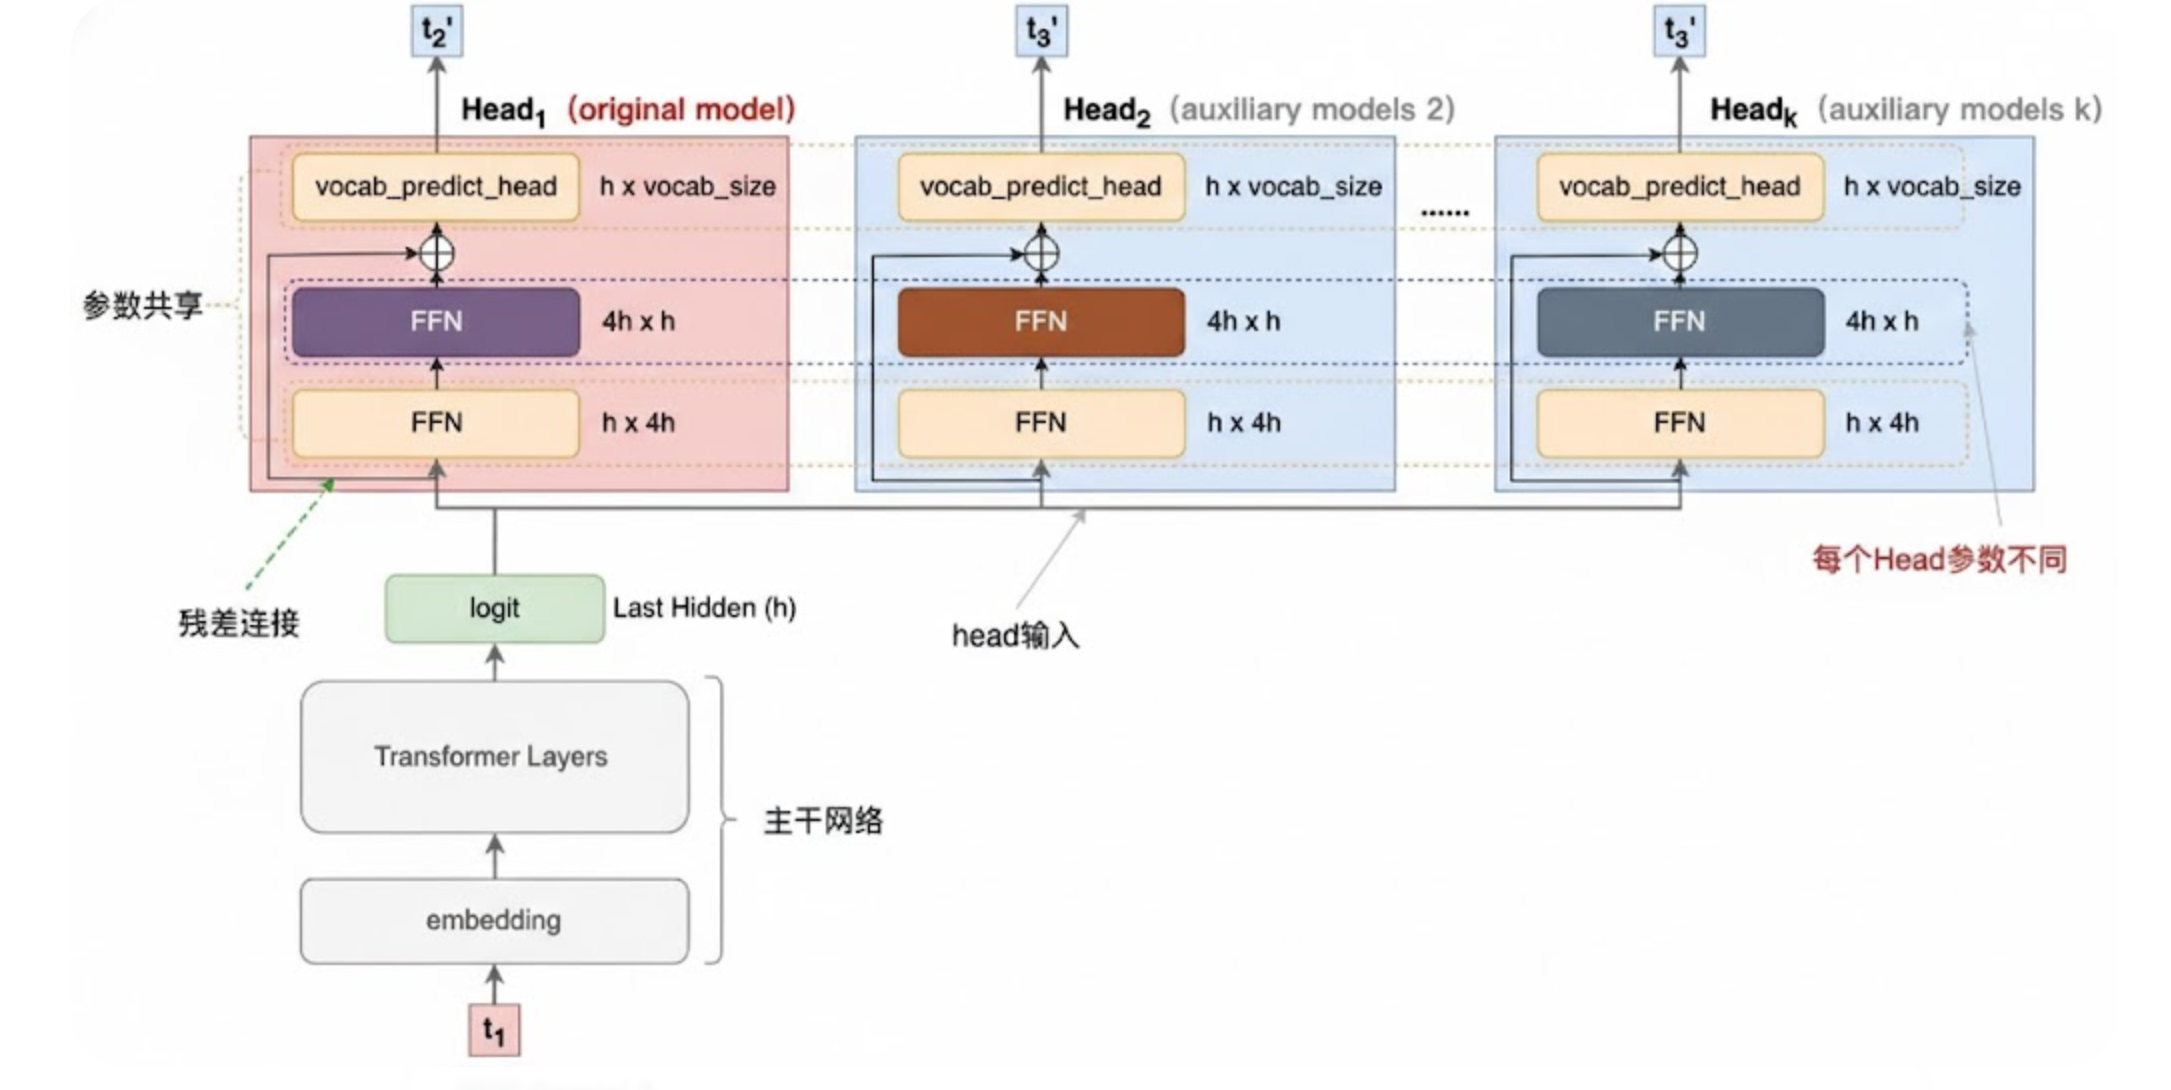
\includegraphics{images/image-0022.png}
\caption{Blockwise Parallel Decoding 模型架构图}
\end{figure}

如图，主干网络是训练好的多层decode-only的Transformer网络，经过多层前向计算后，最终隐藏层输出h维度（＝embedding维度）的logit。上面接了多个输出Head，每个Head负责预估一个token。每个Head有三层：首先是一个共享的FFN层，将logit做宽映射（h维-\textgreater4h维）；然后再过一个非共享的FFN层，将logit维度还原（4h维-\textgreater h维），经残差连接，得到h维embedding向量。最后，再将结果送入到词表投影层得到每个词的概率分布。

\begin{enumerate}
\def\labelenumi{\arabic{enumi}.}
\setcounter{enumi}{1}
\tightlist
\item
  生成范式
\end{enumerate}

\begin{figure}[htbp]
\centering
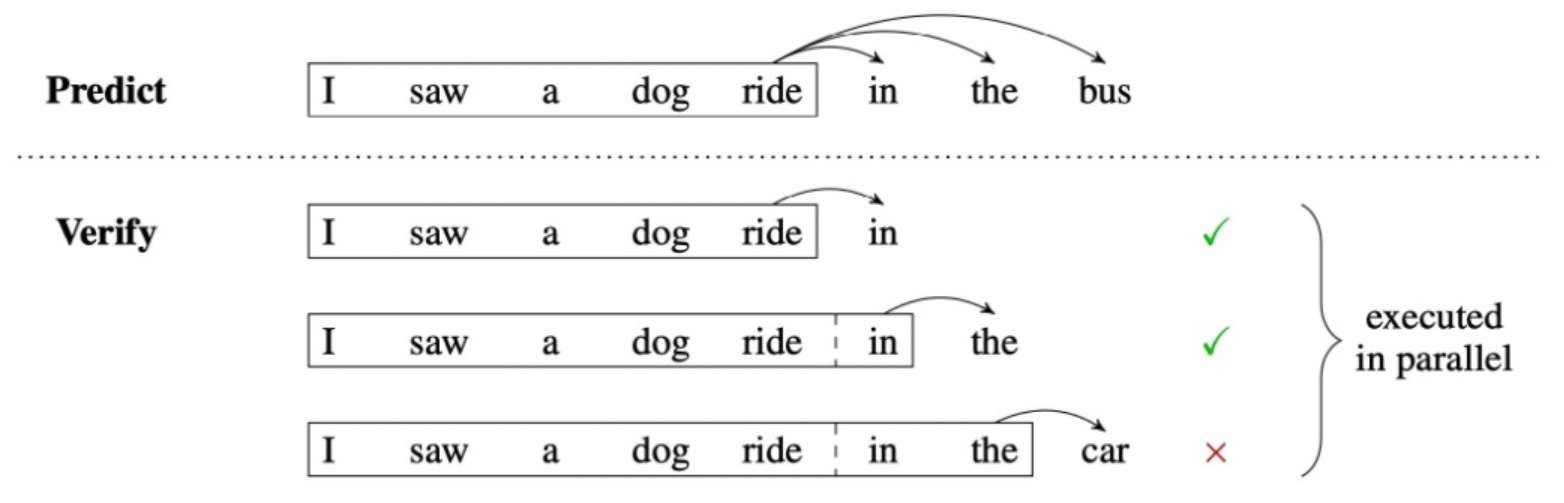
\includegraphics{images/image-0023.png}
\caption{Blockwise Parallel Decoding 的 Predict-Verify 生成与验证流程图}
\end{figure}

MTP的生成过程是一个``Predict-Verify''的循环过程。先一次性预测 \(K\) 个 token，然后利用Transformer的并行性，如图通过掩码的方式实现并行验证。如果预测全部正确，相当于用2次推理的时间实现了 \(K\) 次推理。

进一步地，重叠第 \(n\) 步的 verify 阶段和第 \(n+1\) 步的 predict 阶段，能进一步提高推理性能。如图，先预测出 3 个 token，然后在验证阶段，仍然每次都预测 3 个 token。如由于第 2 个正确，可以以其为条件生成第 3 个``car''、第 4 个``this''和第 5 个``week''，由于最初预测的第 3 个对不上，故最初的预测只能留下``in''和``the''，然后这里生成的第 3 到第 5 个 token 就可以直接作为新的一轮预测，后续再验证此时生成的第 4 和第 5 个，以此类推，不需要重新预测 3 个 token。

\begin{figure}[htbp]
\centering
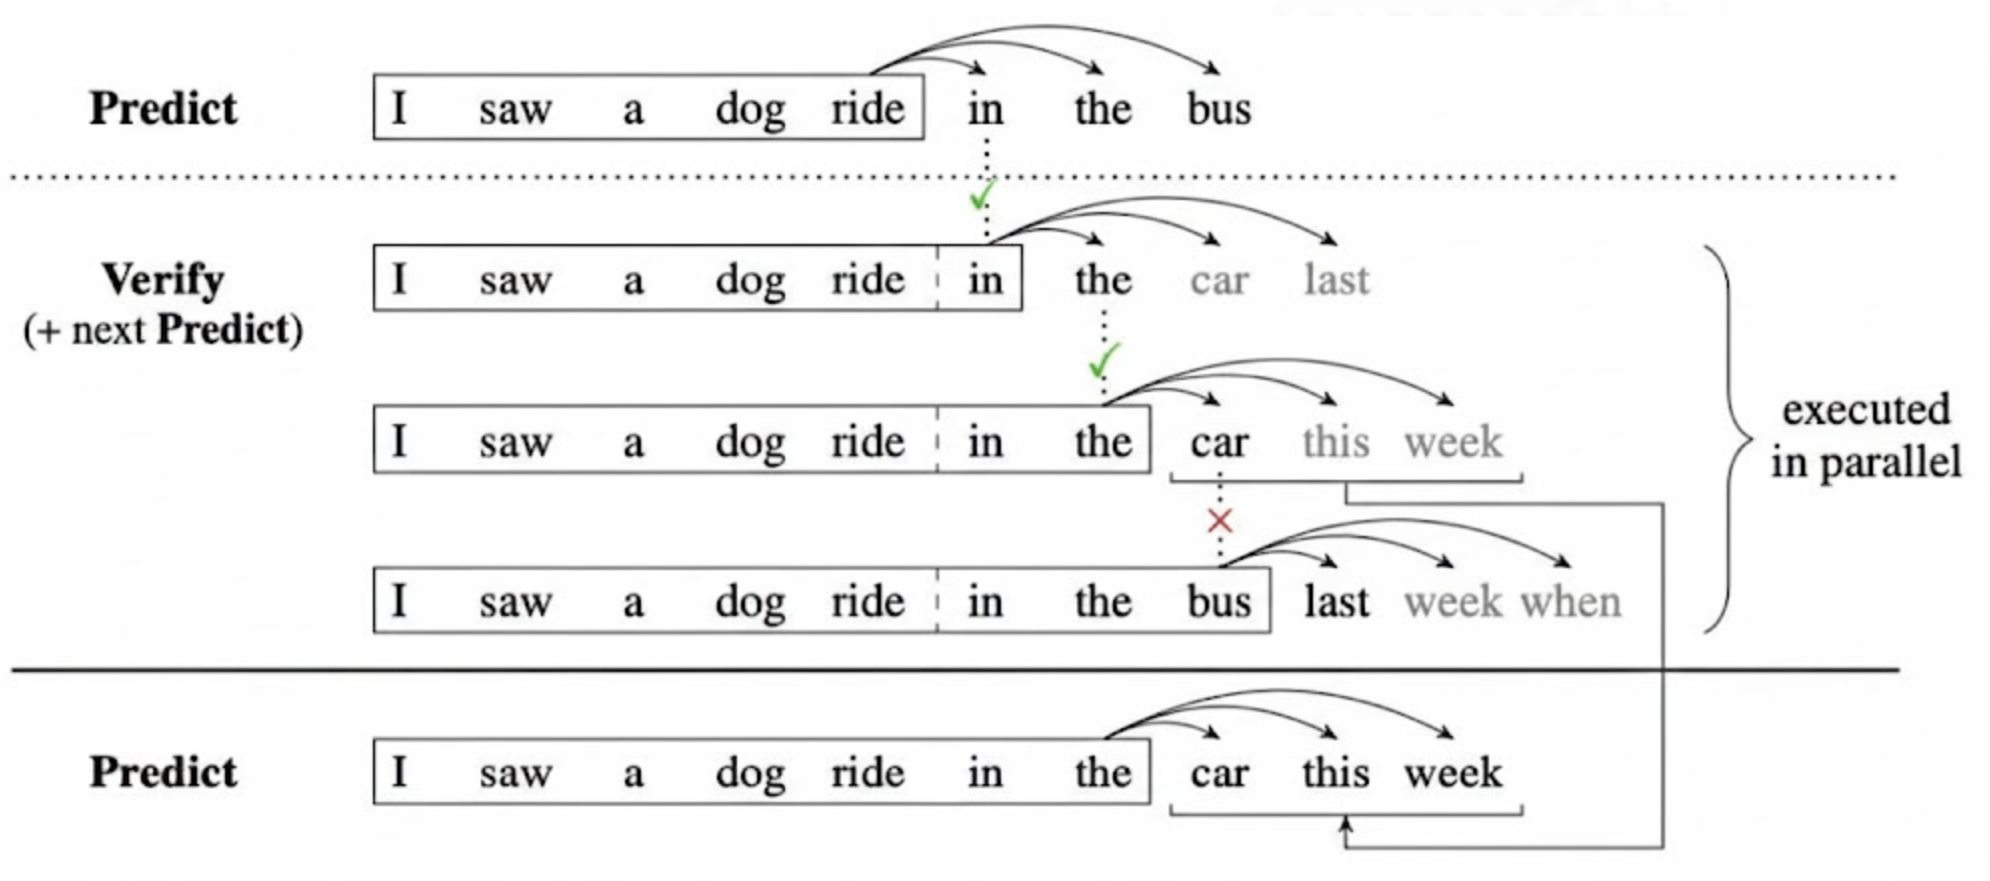
\includegraphics{images/image-0024.png}
\caption{Verify 与下一轮 Predict 重叠执行流程图}
\end{figure}

本质上，这就是利用多token生成的并行性，把后续根据``in''``the''这两个正确的token进行新一轮预测的步骤并入之前的验证步骤。

\hypertarget{ux4e09metas-mtp}{%
\subsection{三、Meta's MTP}\label{ux4e09metas-mtp}}

如图，Meta让每个头不仅仅是FFN层，还有Transformer层，从而可以处理更复杂的序列上下文关系。

\begin{figure}[htbp]
\centering
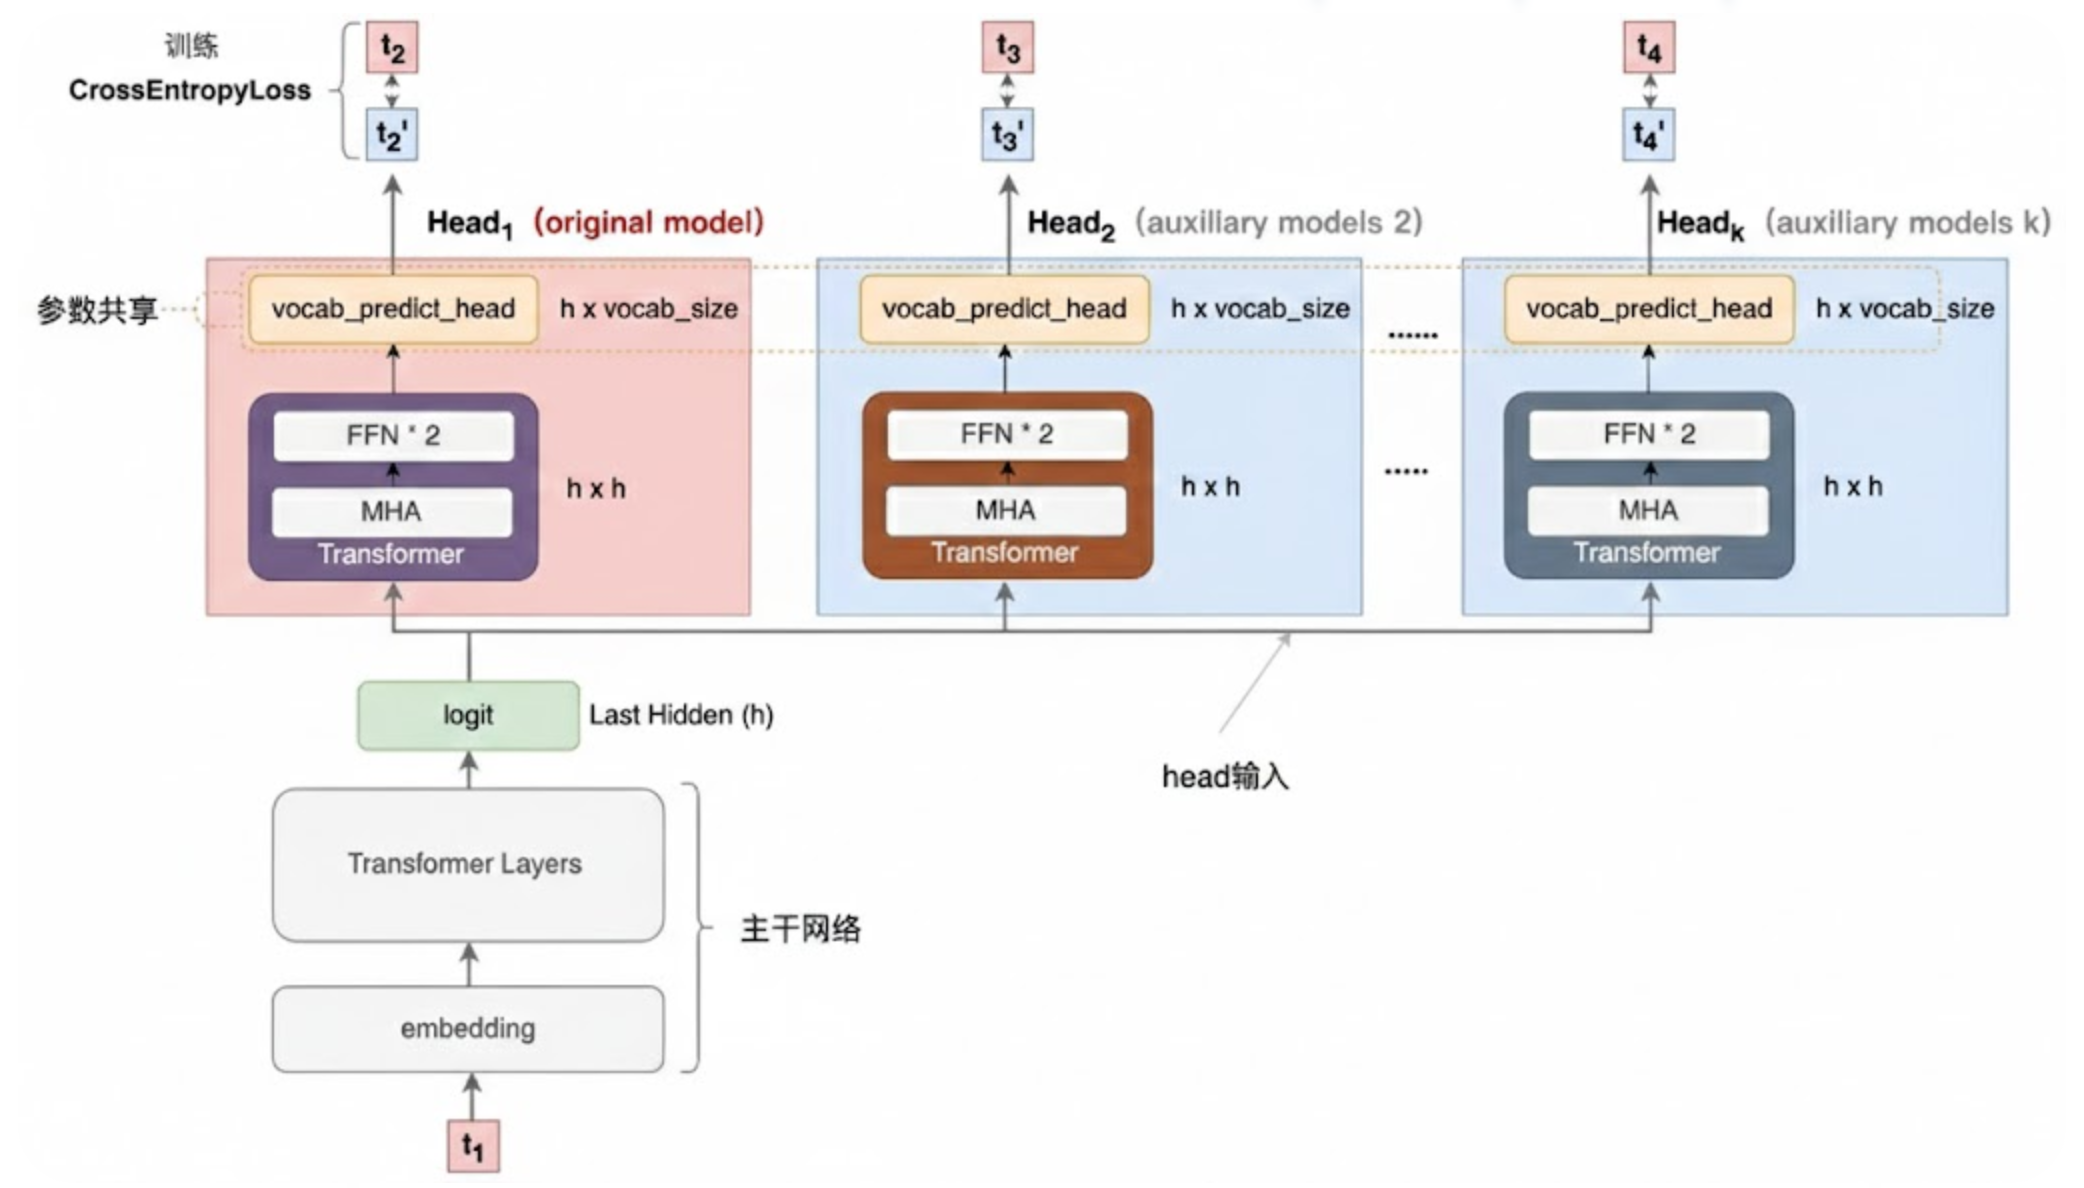
\includegraphics{images/image-0025.png}
\caption{Meta 的 Multi-token Prediction 架构图}
\end{figure}

\hypertarget{ux56dbdeepseek-mtp}{%
\subsection{四、DeepSeek MTP}\label{ux56dbdeepseek-mtp}}

\begin{figure}[htbp]
\centering
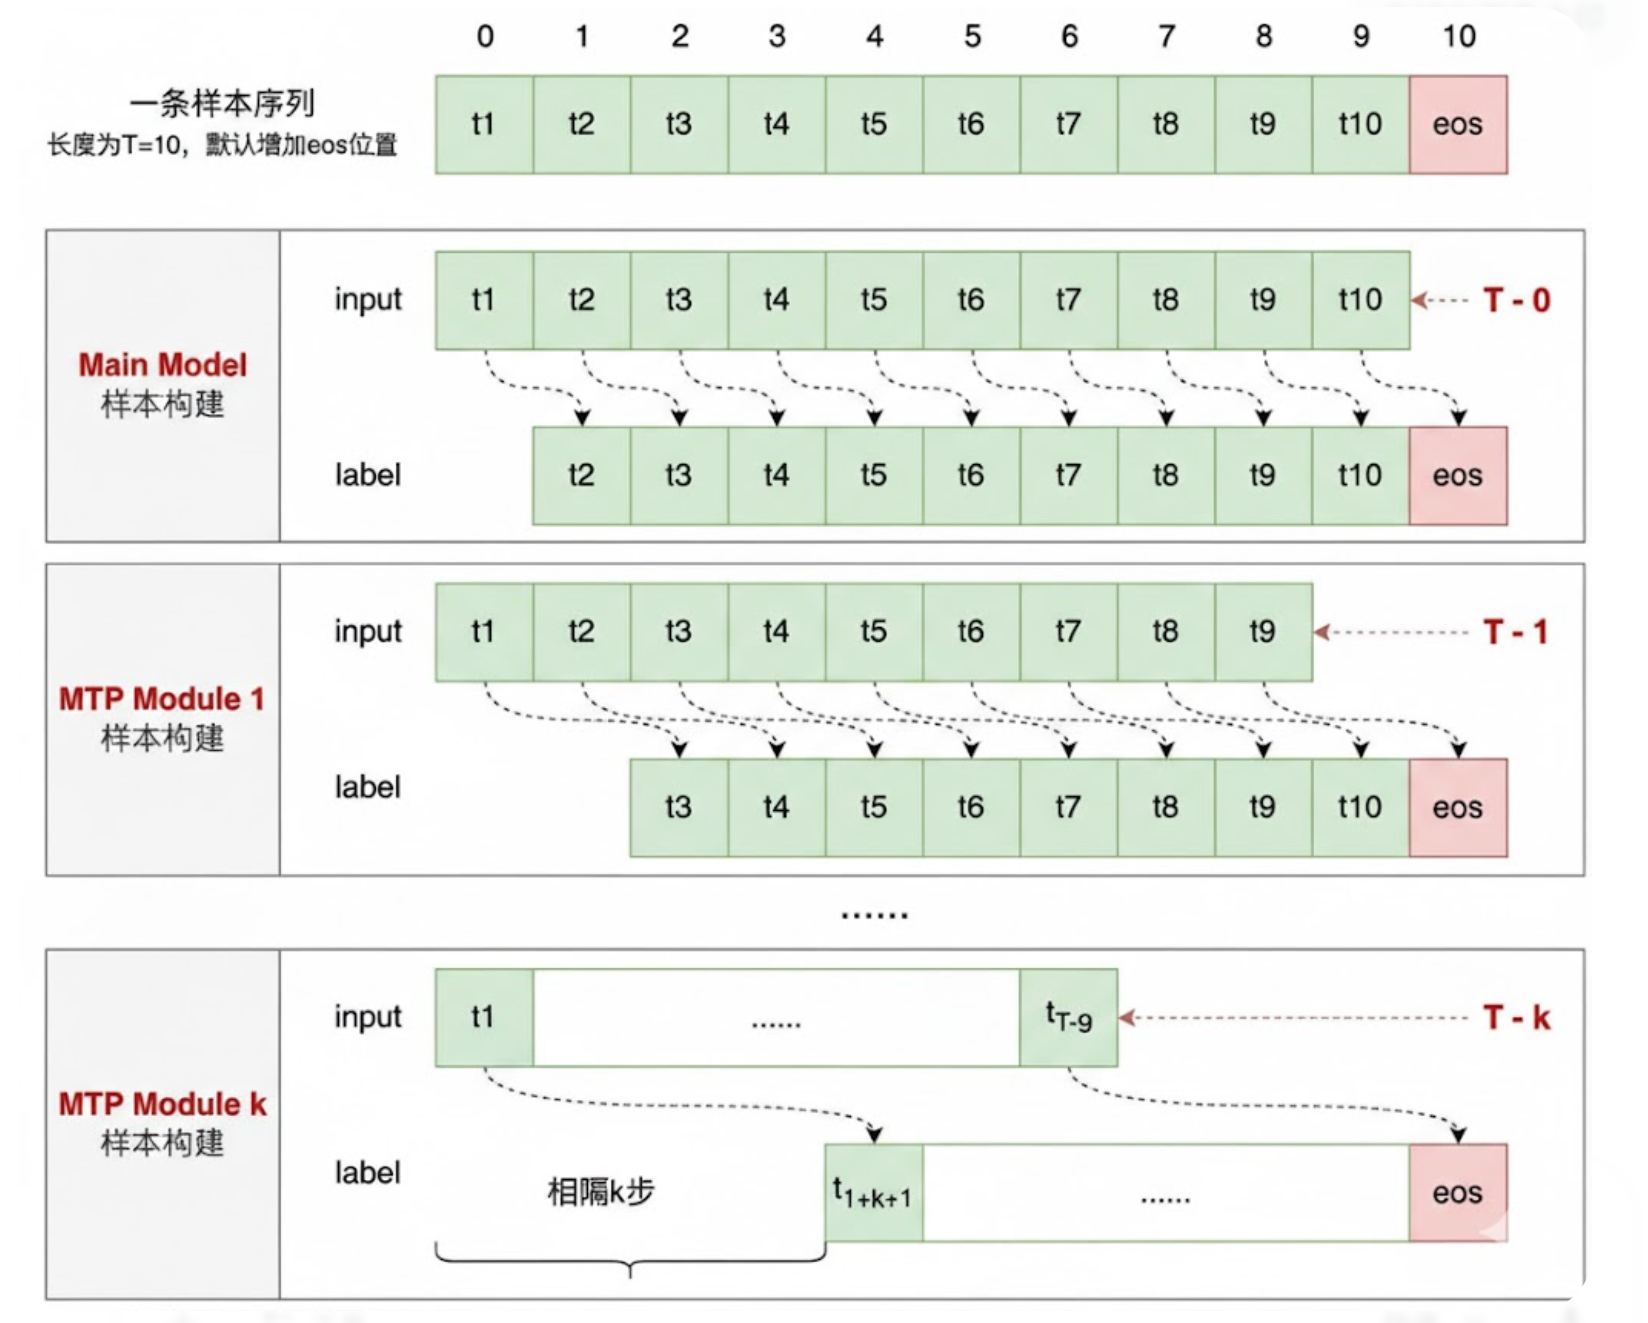
\includegraphics{images/image-0026.png}
\caption{DeepSeek MTP 训练样本构造图}
\end{figure}

训练阶段：Main Model：由 \(t_1\) 生成 \(t_2\)；由 \(t_1,t_2\) 生成 \(t_3\)；\ldots\ldots；由 \(t_1\) 到 \(t_{10}\) 生成 eos token；计算平均Cross-Entropy Loss。MTP Model 1：MTP Module：由 \(t_1,t_2\) 生成 \(t_3\)；\ldots\ldots；由 \(t_1\) 到 \(t_9\) 生成 eos token；计算平均Cross-Entropy Loss。后续的MTP Module以此类推。

\begin{figure}[htbp]
\centering
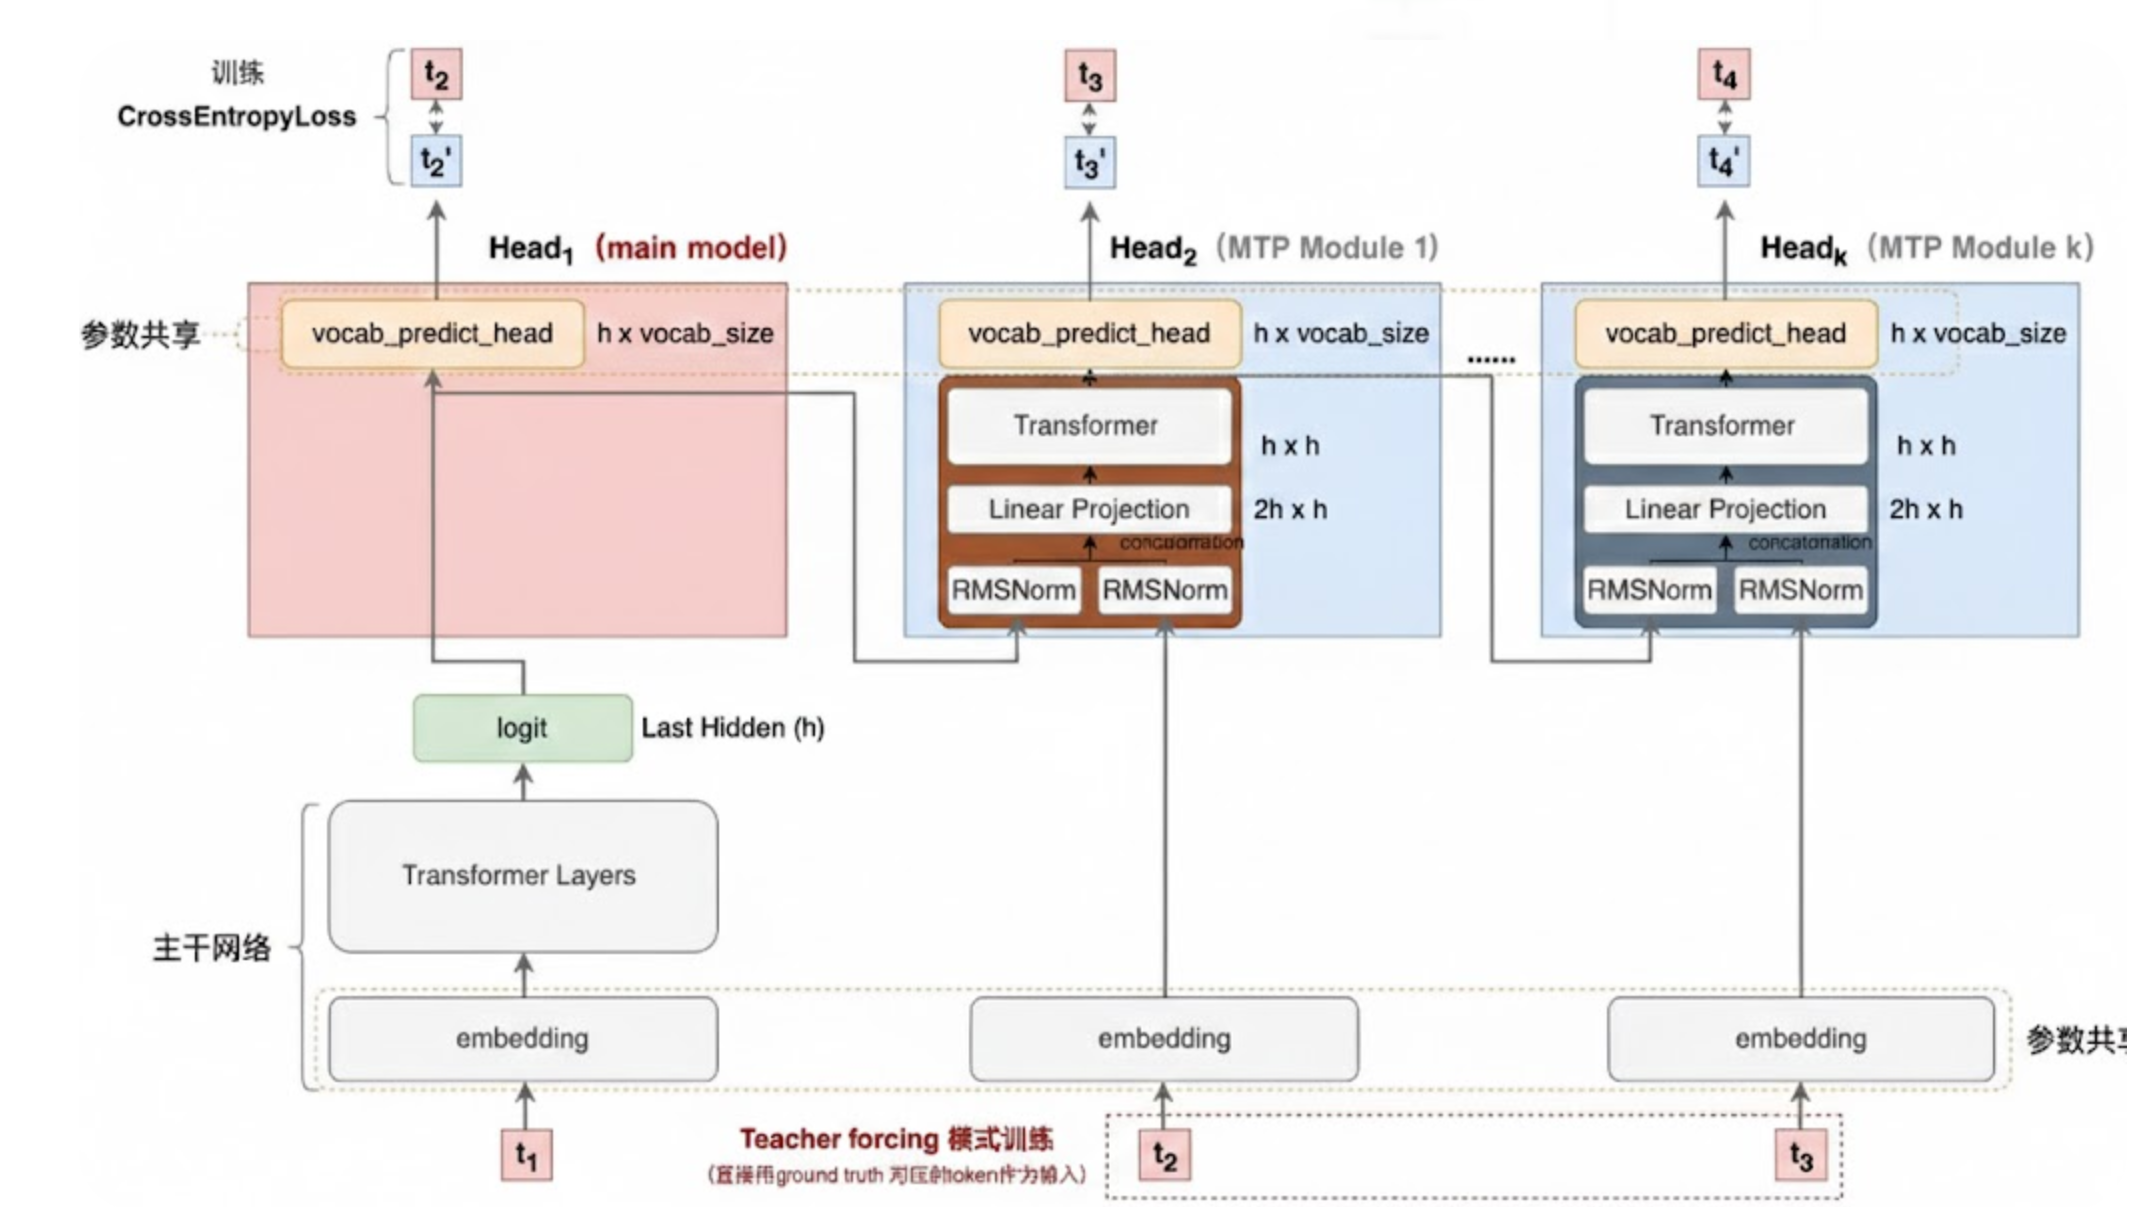
\includegraphics{images/image-0027.png}
\caption{DeepSeek MTP 模块架构图}
\end{figure}

从模型架构上看，DeepSeek在Meta工作的基础上，还在MTP的Transformer层前加上了额外的输入。这个额外输入在训练时是ground truth的t2和t3，以防止细微误差导致``跑偏''；在推理时则是模型自身预测的t2和t3（虽然运用了上一次预测，但这里并非退化为Next token prediction，因为自身预测的t2和t3只经过轻量级MTP模块，不经过全模型，故仍为MTP）。MTP头的损失：

\[
\mathcal{L}_{\mathrm{MTP}}^k
= \mathrm{CrossEntropy}\left(P^k_{2+k:T+1}, t_{2+k:T+1}\right)
= -\frac{1}{T}\sum_{i=2+k}^{T+1}\log P_i^k[t_i].
\]

DeepSeek原论文中插图如下：

\begin{figure}[htbp]
\centering
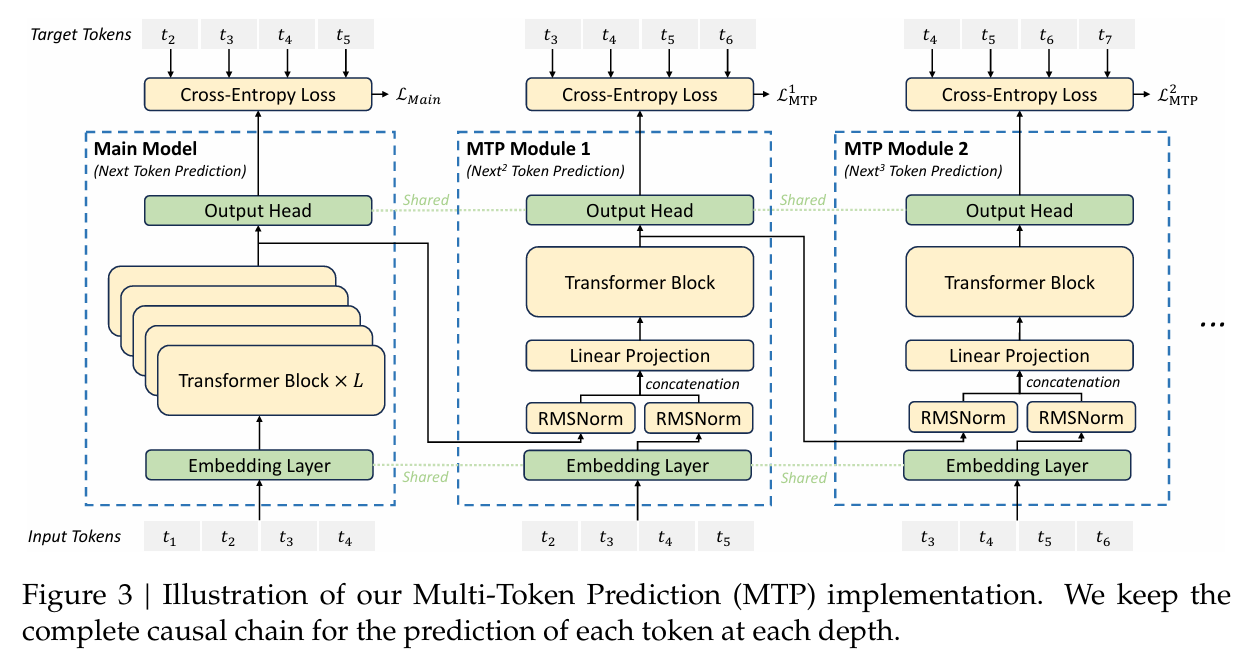
\includegraphics{images/image-0028.png}
\caption{DeepSeek 原论文中的 MTP 模块结构图}
\end{figure}

\hypertarget{ux53c2ux8003ux6587ux732e-99}{%
\subsection{参考文献}\label{ux53c2ux8003ux6587ux732e-99}}

\begin{itemize}
\tightlist
\item
  Stern, M., Shazeer, N., \& Uszkoreit, J. (2018). \href{https://arxiv.org/abs/1811.03115}{Blockwise Parallel Decoding for Deep Autoregressive Models}. NeurIPS 2018.
\item
  Gloeckle, F., Idrissi, B. Y., Roziere, B., et al.~(2024). \href{https://arxiv.org/abs/2404.19737}{Better \& Faster Large Language Models via Multi-token Prediction}. ICML 2024.
\item
  DeepSeek-AI. (2024). \href{https://arxiv.org/abs/2412.19437}{DeepSeek-V3 Technical Report}. arXiv:2412.19437.
\item
  姜富春. (2025). \href{https://zhuanlan.zhihu.com/p/18056041194}{从DeepSeek V3的MTP，解析MTP技术的前世今生}. 知乎专栏.
\end{itemize}

\clearpage

\hypertarget{engramux6a21ux5757ux8bbaux6587}{%
\section{Engram模块（论文）}\label{engramux6a21ux5757ux8bbaux6587}}

\begin{quote}
本文是论文阅读笔记，内容代表对应论文方法或作者理解，不应直接视为领域共识或工程最佳实践。
\end{quote}

传统的大模型架构缺少原生的知识查找方式，只能通过多层计算来低效地模拟检索。如前文为``The capital of France is''时，无法直接查找出``Paris''，只能通过大量参数计算得出。Engram基于条件记忆（Conditional Memory）机制，将记忆（静态知识）与计算（推理能力）解耦，基于哈希查找实现了一种高效率的知识存取方式，从而将更多参数层``腾出来''用于推理。

由于单个token级别的语义记忆在embedding中，跨越上下文的语义通过Attention推理优于直接记忆，故Engram解决的实际上是2-3个token构成的``短语''的记忆问题。

\hypertarget{ux4e00engramux6a21ux5757ux7684ux57faux672cux539fux7406}{%
\subsection{一、Engram模块的基本原理}\label{ux4e00engramux6a21ux5757ux7684ux57faux672cux539fux7406}}

所谓的``静态知识库''实际上是一个长度为S的哈希表，用于存储词组对应的Embedding向量，参数量为S*d\_model。和常见的哈希表初始化为空不同，Engram模块的哈希表初始化时表内的值（参数）均为随机值，后续运用梯度下降更新。研究证明，在模型总参数一定的情况下，除去维度固定的Attention模块外，其余参数20％-30％分配给静态记忆，70％-80％分配给MoE最优。

Engram模块基于NLP中的N-gram方法，N取2和3。推理时，如前文最后三个token为``ABC''时，从哈希表中找2-gram``BC''和3-gram``ABC''对应的几个Engram语义向量，再通过门控机制，按合适的权重加权，加到原向量上。

N取2和3是因为，N=2和N=3覆盖了绝大多数的固定搭配、短语、成语和专有名词（如``New York''``Machine Learning''），这是静态记忆收益最高的区间。N=1对应的是单个词，已经由 Transformer最底层的Embedding Layer完成了，没必要重复存储；N增大，可能的组合呈指数级增长（V\^{}N），但实际在语料中出现的频率却急剧下降，且长序列通常包含复杂的逻辑结构，这部分更适合交给Attention机制动态推导，而不是死记硬背。

\begin{figure}[htbp]
\centering
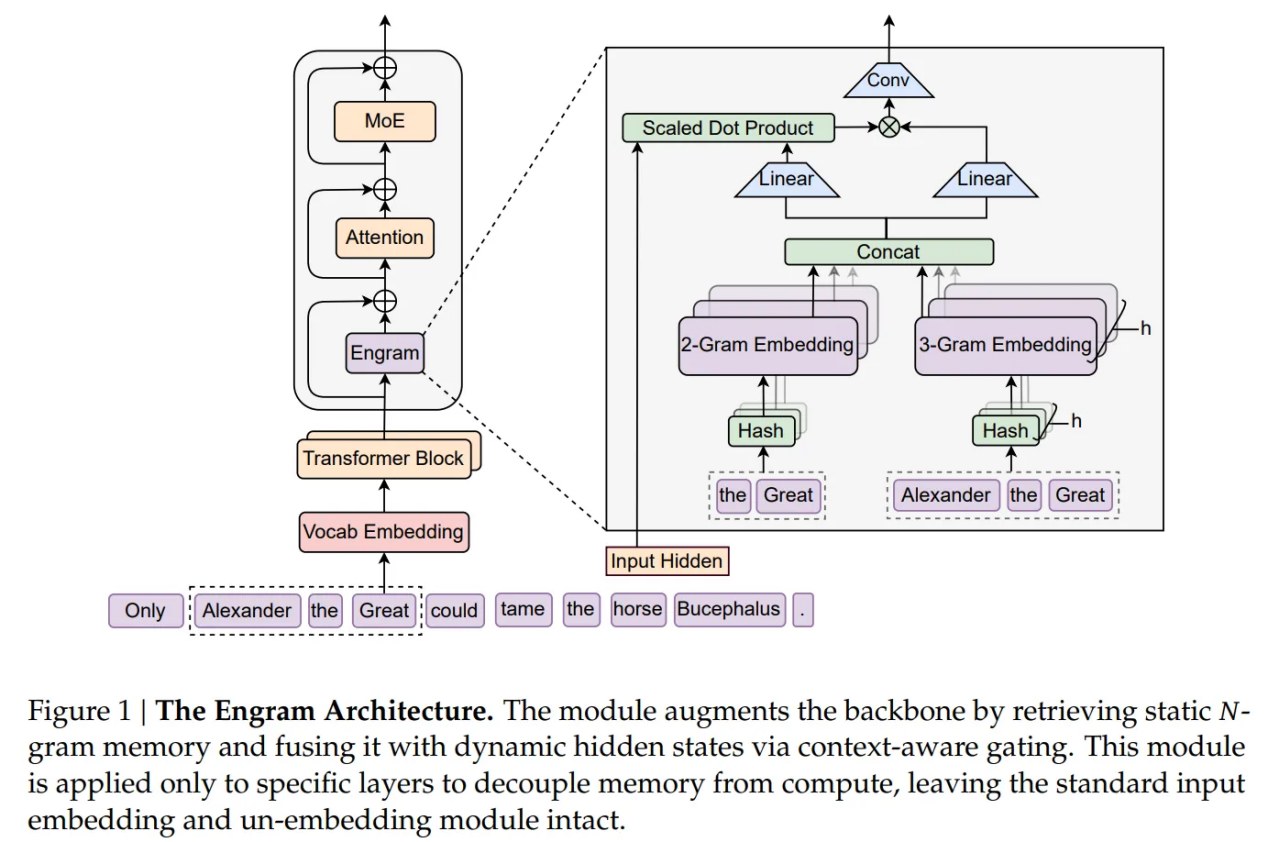
\includegraphics{images/image-0029.png}
\caption{Engram 模块架构图}
\end{figure}

\hypertarget{ux4e8cux54c8ux5e0cux67e5ux627e}{%
\subsection{二、哈希查找}\label{ux4e8cux54c8ux5e0cux67e5ux627e}}

对于输入token序列（为了让查表更紧凑，模型首先将token ID映射到规范形式，如Token ID 105 (``The'')和Token ID 203 (``the'')映射到同一个ID，减少有效词表大小），对于当前第i个token，系统提取其前缀的N-gram，多头哈希函数H\_k计算出K个不同的索引，分别提取这K个位置的Embedding向量。取K个不同的索引是为了缓解哈希冲突，如N-gram A映射到 {[}42, 88{]}，N-gram B映射到 {[}42, 15{]}，42号槽位发生了冲突（Dirty），它混合了A和B的特征，变成了噪声，训练会让模型学会``信任''干净的槽位，而忽略那个冲突的槽位。

如果不用多头，为了避免冲突，必须把表开得非常非常大；使用了多头哈希，可以用一个相对较小（比如S=1亿）的表，容忍一定的碰撞，只要有干净的即可。

\hypertarget{ux4e09ux95e8ux63a7ux673aux5236}{%
\subsection{三、门控机制}\label{ux4e09ux95e8ux63a7ux673aux5236}}

查找得到向量后，将它们与原始输入向量进行门控加和。门控机制类似于一个去掉Softmax的小型Cross-Attention模块，可以根据输入语境确定每个查找到的向量以多大权重聚合进来。由输入向量得到Q、Engram向量矩阵得到K和V，Q和K点乘也就是根据输入决定每个维度的权重分数（这里是独立计算每个向量注入的权重，故不归一化），然后再将每个检索得到的V向量按权重加权得到Engram\_Output向量。最后与原输入向量相加：h\_\{next\} = h\_\{input\} + Engram\_Output。

如输入``capital of France''，模型处于``知识饥渴''状态，查表得到的``Paris''对应向量点积分数高（极大化``Paris''作为下一个词出现的概率），因哈希冲突查到的无关的``Apple''对应向量点积分数低，结果``Paris''相关向量被强力注入，辅助预测；代码推理任务下，所有向量所有维度权重几乎全0，相当于将Engram模块旁路。

\hypertarget{ux56dbux548cux786cux4ef6ux7684ux534fux540cux6027}{%
\subsection{四、和硬件的协同性}\label{ux56dbux548cux786cux4ef6ux7684ux534fux540cux6027}}

\begin{enumerate}
\def\labelenumi{\arabic{enumi}.}
\item
  异步计算和存储：在训练时，为便于反向传播梯度，Engram模块分布在多块GPU上；在推理时，则存储在CPU上，在GPU进行前几层Attention计算时，CPU也在根据输入序列的token ID进行哈希查找，找到N-gram向量，到GPU执行到需要检索的步骤时完成门控嵌入即可。
\item
  分层设计：自然语言中的N-gram 遵循Zipfian分布，即少量高频模式贡献了绝大多数的记忆访问，故可以构建一种多级缓存层次结构（Multi-Level Cache Hierarchy）：将高频访问的嵌入缓存于更快的存储介质中（如GPU HBM或主机DRAM），而将大量低频的长尾模式存放在容量更大但速度较慢的存储介质中（如NVMe SSD）。这种分层设计使Engram能够扩展到极大规模的记忆容量，同时对有效访问延迟的影响保持在最低水平。
\end{enumerate}

\hypertarget{ux53c2ux8003ux6587ux732e-100}{%
\subsection{参考文献}\label{ux53c2ux8003ux6587ux732e-100}}

\begin{itemize}
\tightlist
\item
  Cheng, X., Zeng, W., Dai, D., et al.~(2026). \href{https://arxiv.org/abs/2601.07372}{Conditional Memory via Scalable Lookup: A New Axis of Sparsity for Large Language Models}. arXiv:2601.07372.
\end{itemize}

\clearpage

\hypertarget{ux6d41ux5f62ux5047ux8bbeux4e0eux8d85ux8fdeux63a5}{%
\section{流形假设与超连接}\label{ux6d41ux5f62ux5047ux8bbeux4e0eux8d85ux8fdeux63a5}}

\hypertarget{ux4e00ux6d41ux5f62ux5047ux8bbe}{%
\subsection{一、流形假设}\label{ux4e00ux6d41ux5f62ux5047ux8bbe}}

虽然数据嵌入在一个高维的欧氏空间中，但有意义的数据分布实际上集中在一个维数低得多的低维流形上。也就意味着，对于一个神经网络（或其局部块），从输入x到输出y之间经过的变换是低维的，y-x是分布在低维空间内的向量。

Yoshua Bengio团队在论文《Representation Learning: A Review and New Perspectives》中指出，深度神经网络之所以能泛化，是因为它们成功地学习到了数据所在的低维流形结构，并将其``展开''到了平坦的特征空间中。

\hypertarget{ux4e8cux8d85ux8fdeux63a5hyper-connectionshc}{%
\subsection{二、超连接（Hyper Connections，HC）}\label{ux4e8cux8d85ux8fdeux63a5hyper-connectionshc}}

\hypertarget{ux4e00ux6269ux5c55ux6b8bux5deeux6d41ux5bbdux5ea6}{%
\subsubsection{（一）扩展残差流宽度}\label{ux4e00ux6269ux5c55ux6b8bux5deeux6d41ux5bbdux5ea6}}

在传统的残差神经网络中，y=f(x)+x，f(x)是神经网络主体函数。这里f(x)的输入和输出维度均和x、y的维度相同，均为d\_model。但实际上，f(x)的有效维度应该远小于x、y的表征维度，因此传统的残差神经网络x与y之间的``信息高速公路''太窄，``损失''了很多x、y的有效表征维度，还容易引起网络训练不稳定。

为此，HC将残差流的维度（信息传输维度）和网络主体函数f的维度（计算维度）解耦，加大了残差流的维度，并引入可学习的降维矩阵Hl\_pre和升维矩阵Hl\_post，完成残差流维度和计算维度之间的转换，从而在不显著增大总参数量的前提下，显著增大实际能承载的信息量。

\begin{figure}[htbp]
\centering
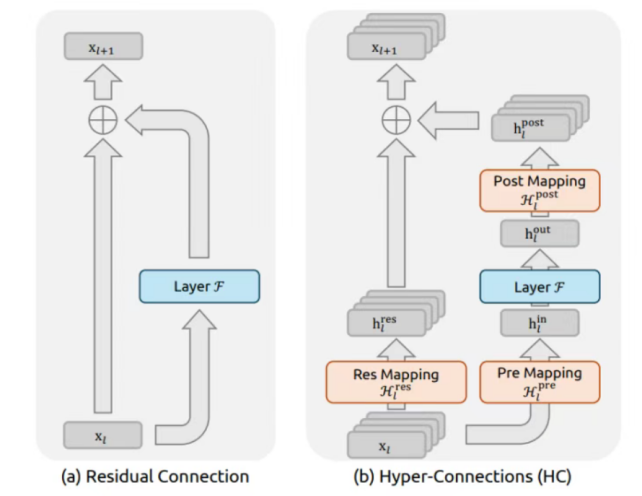
\includegraphics{images/image-0030.png}
\caption{残差连接与超连接结构对比图}
\end{figure}

\hypertarget{ux4e8cux5f15ux5165ux53efux5b66ux4e60ux7684ux6b8bux5deeux8fdeux63a5ux77e9ux9635}{%
\subsubsection{（二）引入可学习的残差连接矩阵}\label{ux4e8cux5f15ux5165ux53efux5b66ux4e60ux7684ux6b8bux5deeux8fdeux63a5ux77e9ux9635}}

从理论上讲，前面的做法已经比较完备了。但HC还引入了残差连接矩阵Hl\_res，对残差流进行线性变换。原因：

\begin{enumerate}
\def\labelenumi{\arabic{enumi}.}
\item
  更好地拟合弯曲流形：深度神经网络由多层构成，对于任意的l，第l层的输出x\_l+1和输入x\_l之差确实都分布在低维空间中，但每一层对应的低维空间的取向往往有一定差异，现实中它们构成的整体流形在高维空间中往往是弯曲的。引入可学习的残差连接矩阵可以让函数的高维空间基底向量灵活地旋转（即不同维度之间可以发生信息交换），增强拟合弯曲流形的性能。
\item
  引入遗忘机制：早期的特征（比如第一层的边缘纹理）在第100层可能已经完全没用了，变成了噪音，但如果不引入Hl\_res，它很难被去除，只能被后面的层通过LayerNorm强行压制，这会浪费宝贵的动态范围。当Hl\_res的特征值小于1时，它起到了遗忘机制的作用。
\end{enumerate}

\hypertarget{ux4e09ux6d41ux5f62ux7ea6ux675fux8d85ux8fdeux63a5}{%
\subsection{三、流形约束超连接}\label{ux4e09ux6d41ux5f62ux7ea6ux675fux8d85ux8fdeux63a5}}

流形约束超连接（Manifold-Constrained Hyper-Connections，mHC）由DeepSeek于2026年提出，是对HC的重要工程化改进。

\hypertarget{ux4e00hcux5b58ux5728ux7684ux95eeux9898}{%
\subsubsection{（一）HC存在的问题}\label{ux4e00hcux5b58ux5728ux7684ux95eeux9898}}

\begin{enumerate}
\def\labelenumi{\arabic{enumi}.}
\item
  数值不稳定：原始的HC中，连接矩阵没有额外的约束，信号在经过多层传播后容易发生梯度爆炸（可达到数百甚至上千倍）或梯度消失，且这还破坏了恒等映射的特性。
\item
  显存和通信开销大：通道变宽意味着显存读写（I/O）和通信成本大幅度增加，即``显存墙''问题。
\end{enumerate}

\hypertarget{ux4e8cmhcux7684ux6539ux8fdb}{%
\subsubsection{（二）mHC的改进}\label{ux4e8cmhcux7684ux6539ux8fdb}}

mHC将变换Hl\_res，Hl\_pre和Hl\_post均限制在了特定的流形上。

\begin{enumerate}
\def\labelenumi{\arabic{enumi}.}
\tightlist
\item
  将Hl\_res限制为双拟随机矩阵
\end{enumerate}

利用Sinkhorn-Knopp 算子，将Hl\_res限制为各元素非负、每行和为1、每列和为1的双拟随机矩阵。本质上说，双拟随机矩阵是排列矩阵的凸组合（排列矩阵：每行、每列只有一个1，其他均为0，一个矩阵乘以排列矩阵，等价于将原矩阵的特征维度向量交换位置），在几何上也就意味着``对于输入向量进行多种旋转（加权）''。它的重复应用会单调地增加跨流的特征融合和信息混合。

此外，该方法在工程上还有两方面优点：

（1）其2-范数有界且不超过1，学习到的映射是非扩张的，可有效缓解梯度爆炸问题。

（2）双拟随机矩阵集对矩阵乘法具有封闭性，确保了跨多层的复合残差映射仍保持双拟随机，从而可在整个模型深度上维持稳定性。

\begin{figure}[htbp]
\centering
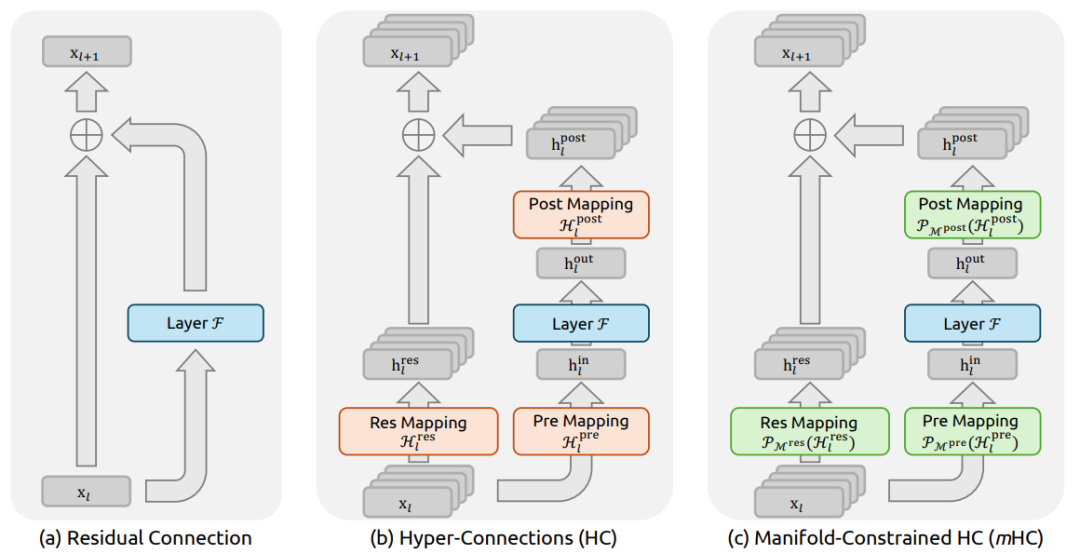
\includegraphics{images/image-0031.png}
\caption{残差连接、超连接与流形约束超连接结构对比图}
\end{figure}

\begin{enumerate}
\def\labelenumi{\arabic{enumi}.}
\setcounter{enumi}{1}
\tightlist
\item
  对Hl\_pre和Hl\_post施加非负约束
\end{enumerate}

Hl\_pre是一个特征重组矩阵，调节各个特征的信号。其第i行第j列的值代表：用于本层计算的低维特征中的第i个维度中，来自高维特征中第j个维度的权重。mHC对两个矩阵均用sigmoid函数转换以保证非负性，提高稳定性，避免正负参数抵消。

注意：这里不用Softmax，因为Softmax要求每行权重之和为1。Hl\_pre如果为10000*1000维，则Softmax会导致输入总信号减小10倍（单个维度信号大小数量级不变，维度除以10）。作为一个门控机制的实现模块，这是不可接受的。

\hypertarget{ux53c2ux8003ux6587ux732e-101}{%
\subsection{参考文献}\label{ux53c2ux8003ux6587ux732e-101}}

\begin{itemize}
\tightlist
\item
  Zhu, D., et al.~(2025). \href{https://arxiv.org/abs/2409.19606}{Hyper-Connections}. arXiv:2409.19606.
\item
  DeepSeek-AI. (2025). \href{https://arxiv.org/abs/2512.24880}{mHC: Manifold-Constrained Hyper-Connections}. arXiv:2512.24880.
\end{itemize}

\clearpage

\hypertarget{attention-residualsux8bbaux6587}{%
\section{Attention Residuals（论文）}\label{attention-residualsux8bbaux6587}}

\begin{quote}
本文是论文阅读笔记，内容代表对应论文方法或作者理解，不应直接视为领域共识或工程最佳实践。
\end{quote}

\hypertarget{ux4e00ux95eeux9898ux80ccux666f-1}{%
\subsection{一、问题背景}\label{ux4e00ux95eeux9898ux80ccux666f-1}}

主流大模型内部的残差连接在每一层处理完信息之后，把处理结果和原来的输入加在一起，传给下一层。每一层做完累加之后，信息就被压进了一个混合状态里。越往后，这个混合状态就越臃肿。随着网络越来越深，混合状态的数值越来越大，发生PreNorm稀释：越深的层，贡献越被稀释。实验证明，一个很深的模型里，删掉相当多的层，效果几乎不变。我们实际上浪费了大量算力。

\hypertarget{ux4e8cux6838ux5fc3ux601dux60f3-1}{%
\subsection{二、核心思想}\label{ux4e8cux6838ux5fc3ux601dux60f3-1}}

目前的主流架构中，每一层的输入=网络输入+前面所有层的输出（等权重）。Kimi团队提出，可以让每一层=网络输入+前面所有层的输出（按需加权求和），权重由这一层自己学。

具体而言，就是用注意力机制，让模型自主决定关注哪些层。每一层有一个自己专属的小向量（只有一个，极其轻量），用它去跟前面所有层的输出算相似度，相似度高的层权重就大，相似度低的权重就小，最后加权求和。值得注意的是，注意力层和MLP层可以关注不同的历史层。

这样，早期层的信息就不会被淹没，可以按需取用。整个改动增加的参数量，相比几十亿参数的大模型来说可以忽略不计，但性能提升到原来的1.25倍，相对于同等性能下节省20％算力。

\hypertarget{ux4e09block-attention-residuals}{%
\subsection{三、Block Attention Residuals}\label{ux4e09block-attention-residuals}}

这种方法的工程问题在于，每一层要关注前面所有层的输出，就必须把前面所有层的输出都存着。现代大模型一般有上百层，训练时还会把模型切成很多份分布到不同机器上（流水线并行），每台机器都要维护所有层的输出，内存压力和通信压力都会暴增。

Kimi的解法是，不用存每一层，改为存每一组。把所有层分成若干个块（block），每个块内部还是用传统方式累加，但把整个块压缩成一个向量存起来。跨块之间，再用注意力机制选择。这样存储量从正比于层数，变成正比于块数。实验发现，分成大约8块就能恢复Full Attention Residuals绝大部分的效果，而内存和通信开销只是原来的一小部分。

\hypertarget{ux53c2ux8003ux6587ux732e-102}{%
\subsection{参考文献}\label{ux53c2ux8003ux6587ux732e-102}}

\begin{itemize}
\tightlist
\item
  Moonshot AI. (2026). \href{https://arxiv.org/abs/2603.15031}{Attention Residuals}. arXiv:2603.15031.
\end{itemize}

\clearpage

\hypertarget{ux81eaux84b8ux998f}{%
\section{自蒸馏}\label{ux81eaux84b8ux998f}}

\hypertarget{ux4e00ux57faux4e8eux4e13ux5bb6ux6f14ux793aux7684ux65b9ux6cd5ux81eaux84b8ux998fux5faeux8c03sdft}{%
\subsection{一、基于专家演示的方法：自蒸馏微调（SDFT）}\label{ux4e00ux57faux4e8eux4e13ux5bb6ux6f14ux793aux7684ux65b9ux6cd5ux81eaux84b8ux998fux5faeux8c03sdft}}

\begin{enumerate}
\def\labelenumi{\arabic{enumi}.}
\tightlist
\item
  提出背景
\end{enumerate}

目前，从专家演示中学习的主流范式是监督微调（SFT）。SFT是Off-policy学习，当模型需要顺序适应新任务或新领域时，SFT会导致严重的泛化能力下降和灾难性遗忘现象。虽然On-policy RL可以显著减少遗忘并提升分布外泛化能力，但它通常需要一个明确的奖励函数。在许多现实世界场景中，构建这样精确的奖励函数是非常困难甚至不可用的。

\begin{enumerate}
\def\labelenumi{\arabic{enumi}.}
\setcounter{enumi}{1}
\tightlist
\item
  核心原理
\end{enumerate}

为了在只有演示或环境反馈数据而没有明确奖励函数的情况下获得同策略学习的优势，自蒸馏让同一个模型在训练中同时扮演``教师''和``学生''两个角色。

学生模型仅接收原始的任务提示词并自回归生成；教师模型接收任务提示词和专家演示，通过大模型的上下文学习能力，每次在学生模型的前 \(i-1\) 个token基础上生成包含正确任务意图的第 \(i\) 个token作为高质量指导信号。

学生模型和教师模型对应的分布可以写为：

\begin{itemize}
\tightlist
\item
  学生模型：在给定前缀 \(y_{<t}\) 和原始问题 \(x\) 的情况下，预测下一个词元的概率分布 \(\pi_\theta(\cdot \mid y_{<t}, x)\)。
\item
  教师模型：在同样前缀下，同时接收专家演示增强提示词 \(c\)，给出更高质量的概率分布 \(\pi(\cdot \mid y_{<t}, x, c)\)。
\end{itemize}

其整体序列级别的逆 KL 散度优化目标为：

\[
\mathcal{L}(\theta)
= D_{\mathrm{KL}}\left(\pi_\theta(\cdot \mid x)\,\Vert\,\pi(\cdot \mid x,c)\right)
= \mathbb{E}_{y\sim \pi_\theta(y\mid x)}
\left[
\log\frac{\pi_\theta(y\mid x)}{\pi(y\mid x,c)}
\right].
\]

式外的期望 \(\mathbb{E}_{y\sim \pi_\theta(y\mid x)}\) 表明，采样的数据分布来自学生策略 \(\pi_\theta\)。

这其实意味着我们是在对整个词汇表V中所有可能的下一个词元v遍历求和：

\[
\nabla_\theta D_{\mathrm{KL}}(\pi_\theta\Vert\pi)
=
\sum_{v\in V}
\pi_\theta(v\mid y_{<t})
\nabla_\theta \log \pi_\theta(v\mid y_{<t})
\left(
\log\frac{\pi_\theta(v\mid y_{<t})}{\pi(v\mid y_{<t},c)}
+ 1
\right).
\]

把每个时间步上的词表求和写成解析梯度估计时，需要保留学生分布的概率权重：

\[
\hat{g}_{\mathrm{analytic}}
=
\sum_{t=1}^{T}\sum_{v\in V}
\pi_\theta(v\mid y_{<t},x)
\nabla_\theta \log \pi_\theta(v\mid y_{<t},x)
\left(
\log\frac{\pi_\theta(v\mid y_{<t},x)}{\pi(v\mid y_{<t},x,c)}
+1
\right).
\]

这在物理意义上等同于：学生模型走到任意一步时，看看在这一步全词表所有可能的选项上，自己的概率分布与教师的概率分布有多大差异，并拉近这种差异。

另外，这里的``专家演示''未必要来自外部，也可以是自身根据后来改出的正确答案。可以类似人类在睡眠时巩固一样，和主进程异步地按自己对同一个问题后来得出的正确答案、优秀经验，对最初上下文较少时的错误输出进行纠正。

\hypertarget{ux4e8cux57faux4e8eux73afux5883ux53cdux9988ux7684ux65b9ux6cd5ux81eaux84b8ux998fux7b56ux7565ux4f18ux5316sdpo}{%
\subsection{二、基于环境反馈的方法：自蒸馏策略优化（SDPO）}\label{ux4e8cux57faux4e8eux73afux5883ux53cdux9988ux7684ux65b9ux6cd5ux81eaux84b8ux998fux7b56ux7565ux4f18ux5316sdpo}}

\begin{enumerate}
\def\labelenumi{\arabic{enumi}.}
\tightlist
\item
  提出背景
\end{enumerate}

RL的训练中，我们通常只会给出一个稀疏的标量结果（如``通过：1''或``未通过：0''），掩盖了底层丰富的状态信息，算法只能把整段代码的所有的词元都进行无差别的梯度惩罚，模型很难弄清楚自己到底错在了哪里------是因为某一行语法写错了、逻辑思辨存在漏洞，还是单纯的边界条件没有处理好。我们希望获得更密集的反馈。

\begin{enumerate}
\def\labelenumi{\arabic{enumi}.}
\setcounter{enumi}{1}
\tightlist
\item
  核心原理
\end{enumerate}

学生模型仅根据原始的指令提示，自回归地生成一个解题尝试。送入可验证环境中执行，环境不仅返回分数，还会输出详细的丰富反馈（如报错信息）。权重相同的教师模型根据原始指令+环境反馈，利用强大的上下文学习能力，在学生模型生成序列的每个位置上，预测下一个词元的正确分布（根据看到的环境反馈得出反思，从而可以纠正学生的错误输出），让学生模型通过最小化KL散度（同前面介绍的反向KL）来逼近这个分布。

\begin{enumerate}
\def\labelenumi{\arabic{enumi}.}
\setcounter{enumi}{2}
\tightlist
\item
  SDPO的好处
\end{enumerate}

相比于奖励信号稀疏的RL，SDPO可以精准地为那一个导致错误的词元计算出巨大的梯度，指导模型只去修正真正犯错的地方。原本仅在序列末尾才有的稀疏且单一的标量奖励，被漂亮地转化为了每一个词元生成时的密集指导信号。理论分析证明，这种机制等价于在最大熵强化学习（Maximum Entropy RL）框架下优化由教师定义的隐式奖励。

这种在PyTorch中仅需调用一次 .forward() 就能算出整条序列密集梯度的设计，不仅避开了off-policy带来的偏移，在显存利用率和计算效率上也远超让两个模型各自生成不同长度序列的传统方法。

\hypertarget{ux53c2ux8003ux6587ux732e-103}{%
\subsection{参考文献}\label{ux53c2ux8003ux6587ux732e-103}}

\begin{itemize}
\tightlist
\item
  Shenfeld, I., Damani, M., Hubotter, J., \& Agrawal, P. (2026). \href{https://arxiv.org/abs/2601.19897}{Self-Distillation Enables Continual Learning}. arXiv:2601.19897.
\item
  Xu, H., et al.~(2026). \href{https://arxiv.org/abs/2601.20802}{Reinforcement Learning via Self-Distillation}. arXiv:2601.20802.
\end{itemize}

\clearpage

\hypertarget{ux591aux4e13ux5bb6on-policy-distillation}{%
\section{多专家On-policy Distillation}\label{ux591aux4e13ux5bb6on-policy-distillation}}

DeepSeek-V4采用了多专家On-policy Distillation的方法，先基于预训练模型，用SFT和RL训练多个领域专家，再将其知识蒸馏到统一的学生模型中。

\hypertarget{ux4e00ux9886ux57dfux4e13ux5bb6ux6a21ux578bux8badux7ec3}{%
\subsection{一、领域专家模型训练}\label{ux4e00ux9886ux57dfux4e13ux5bb6ux6a21ux578bux8badux7ec3}}

基于预训练模型，用SFT和GRPO训练一批领域专家模型，领域包括数学、代码、Agent、指令跟随等。业界一般还会给每个领域训练多种推理强度的子版本，分别对应Non-think、Think、Think Max，三种模式在RL时用不同的length penalty和context window。

做Agent类专家时还引入了~Quick Instruction~机制，聊天产品里有很多附加任务，比如判断是否触发搜索、识别意图。传统做法是另一个小模型做这些，导致每次上下文变化，要重新进行预填充。V4 的做法是给输入序列直接附一组special token，每个token对应一个附加任务，复用现成的KV cache，降低首字延迟。

\hypertarget{ux4e8con-policy-distillation}{%
\subsection{二、On-Policy Distillation}\label{ux4e8con-policy-distillation}}

运用On-Policy蒸馏方法，把所有专家的知识融合到统一的学生模型里。相比于Off-policy方法而言，On-policy更能避免灾难性遗忘。具体而言，即让学生在自己生成的轨迹上学习多个专家模型的输出概率分布。

\hypertarget{ux53c2ux8003ux6587ux732e-104}{%
\subsection{参考文献}\label{ux53c2ux8003ux6587ux732e-104}}

\begin{itemize}
\tightlist
\item
  DeepSeek-AI. (2026). \href{https://huggingface.co/deepseek-ai/DeepSeek-V4-Pro/blob/main/DeepSeek_V4.pdf}{DeepSeek-V4: Towards Highly Efficient Million-Token Context Intelligence}. Technical report.
\end{itemize}

\clearpage

\hypertarget{klux6563ux5ea6ux4e0ejsdux6563ux5ea6}{%
\section{KL散度与JSD散度}\label{klux6563ux5ea6ux4e0ejsdux6563ux5ea6}}

在大模型中，KL散度衡量输出概率分布的差异，并非按输出前的隐藏层维度计算，而是在大小为 \(V\) 的词表上计算（因为本质上大模型的输出是离散的tokens）。

\[
D(P\Vert Q)=\sum_{i=1}^{V}p_i\log\frac{p_i}{q_i}
\]

注意：计算困惑度时是对序列中的所有token的概率负对数取平均，而计算KL散度时是在输出一个token时，对词表中的所有词的KL散度取平均，二者取平均的方式不同。

实际研究中，为了让数值更稳定，往往用KL散度的变体------JSD散度，即取 \(P\) 和 \(Q\) 的平均 \(M\)：

\[
M=\frac{1}{2}(P+Q)
\]

JSD散度定义为：

\[
\mathrm{JSD}(P,Q)=\frac{1}{2}\left(D_{\mathrm{KL}}(P\Vert M)+D_{\mathrm{KL}}(Q\Vert M)\right)
\]

其功能和KL类似但不会出现 \(\log\) 内分母为零，例如研究模型中间隐藏层和输出层之间神经元激活值的JSD散度（如果二者维度不同，则投影后再用JSD散度），就可以判断二者分布之间的相似程度大小。

对于LLM，自回归输出 \(n\) 个token的KL散度：

\[
D_{\mathrm{KL}}(P(Y)\Vert Q(Y))
=
\sum_Y P(Y)\log\frac{P(Y)}{Q(Y)}.
\]

由于直接对所有可能的序列求和是不可行的（有 \(V^n\) 种可能），需利用自回归特性将其分解：

\[
D_{\mathrm{KL}}(P(Y)\Vert Q(Y))
=
\mathbb{E}_{Y\sim P}
\left[
\sum_{t=1}^{n}
\left(
\log P(y_t\mid y_{<t})-\log Q(y_t\mid y_{<t})
\right)
\right]
=
\sum_{t=1}^{n}
\mathbb{E}_{Y\sim P}
\left[
\log\frac{P(y_t\mid y_{<t})}{Q(y_t\mid y_{<t})}
\right].
\]

这里的处理难点在于 \(Y\sim P\)，需要考虑整个序列的概率分布。注意到右边的条件概率的条件为 \(y_{<t}\)，对于给定已知的 \(y_{<t}\) 分布，由自回归特性，\(y_t\) 的分布也会随之确定，\(Y=\{y_1,\ldots,y_t\}\) 的分布也就已知。因此可以改写为：

\[
D_{\mathrm{KL}}(P(Y)\Vert Q(Y))
=
\sum_{t=1}^{n}
\mathbb{E}_{y_{<t}\sim P(y_{<t})}
\left[
D_{\mathrm{KL}}\left(P(y_t\mid y_{<t})\Vert Q(y_t\mid y_{<t})\right)
\right].
\]

这意味着，两个序列分布的KL散度，等于每一步条件概率分布之间KL散度的期望之和（期望是基于分布 \(P\) 生成的历史轨迹计算的）。

\hypertarget{ux53c2ux8003ux6587ux732e-105}{%
\subsection{参考文献}\label{ux53c2ux8003ux6587ux732e-105}}

\begin{itemize}
\tightlist
\item
  Kullback, S., \& Leibler, R. A. (1951). \href{https://doi.org/10.1214/aoms/1177729694}{On Information and Sufficiency}. The Annals of Mathematical Statistics, 22(1), 79-86.
\item
  Lin, J. (1991). \href{https://doi.org/10.1109/18.61115}{Divergence measures based on the Shannon entropy}. IEEE Transactions on Information Theory, 37(1), 145-151.
\end{itemize}

\clearpage

\hypertarget{ux56f0ux60d1ux5ea6}{%
\section{困惑度}\label{ux56f0ux60d1ux5ea6}}

困惑度（Perplexity, PPL）是评估语言模型好坏的黄金指标。它的核心思想是：一个好的模型，应该对真实的下一个词赋予很高的预测概率。模型越感到``困惑''，它的预测就越不准，困惑度的值就越高。

\hypertarget{ux4e00ux76f4ux89c2ux7406ux89e3}{%
\subsection{一、直观理解}\label{ux4e00ux76f4ux89c2ux7406ux89e3}}

假设一个完美的语言模型，它总是能 100\% 确定下一个词是什么（即预测概率为 \(1\)）。那么它的困惑度是 \(\exp(0)=1\)。这意味着模型毫不困惑，等价于它每次只有 1 个词的选择（就是那个正确的词）。

一个非常差的模型，比如它总是认为词表中的所有 10 万个词都是等可能的（每个词概率为 \(1/100000\)）。那么它的困惑度就是 100000。这意味着模型非常困惑，等价于它每次都要在 10 万个词里做选择。

一个好的模型的困惑度应该介于 1 和词表大小之间。例如，在 WikiText-2 数据集上，现代模型的困惑度可以降到 20 左右。这意味着每次模型平均是从 20 个词中选一个，比较``确定''接下来会发生什么。

\hypertarget{ux4e8cux6570ux5b66ux8868ux8fbeux4e0eux63a8ux5bfc}{%
\subsection{二、数学表达与推导}\label{ux4e8cux6570ux5b66ux8868ux8fbeux4e0eux63a8ux5bfc}}

困惑度与信息论中的交叉熵（Cross-Entropy）~紧密相关。交叉熵衡量的是模型预测的概率分布与真实的概率分布（这里其实是one-hot分布，即真实词的概率为1，其他为0）之间的差异。事实上，交叉熵损失函数取指数后，就可以视为整个序列的困惑度（``生成该序列时，每次平均从几个token里选一个''）。困惑度的n次方的倒数就是生成该序列的联合概率，最小化困惑度（PPL）在数学上完全等价于最大化模型分配给整个序列的联合概率。

数学推导：

\begin{enumerate}
\def\labelenumi{\arabic{enumi}.}
\tightlist
\item
  起点：序列概率
\end{enumerate}

语言模型的目标是给真实序列 \(W=(w_1,w_2,\ldots,w_N)\) 赋予高概率。根据链式法则，这个概率是所有条件概率的乘积：

\[
P(W)=P(w_1)\prod_{t=2}^{N}P(w_t\mid w_1,\ldots,w_{t-1})
\]

\begin{enumerate}
\def\labelenumi{\arabic{enumi}.}
\setcounter{enumi}{1}
\tightlist
\item
  取对数（为了将连乘变为求和）
\end{enumerate}

直接优化乘积在数学上很麻烦（可能下溢），我们取对数，转化为对数似然（Log-Likelihood）。因为对数函数是单调的，最大化概率乘积等价于最大化对数似然和。

\[
\log P(W)=\log P(w_1)+\sum_{t=2}^{N}\log P(w_t\mid w_1,\ldots,w_{t-1})
\]

\begin{enumerate}
\def\labelenumi{\arabic{enumi}.}
\setcounter{enumi}{2}
\tightlist
\item
  取平均（为了消除长度影响）
\end{enumerate}

为了比较不同长度序列的性能，我们取平均值，得到平均对数似然。

\[
\frac{1}{N}\log P(W)
\]

\begin{enumerate}
\def\labelenumi{\arabic{enumi}.}
\setcounter{enumi}{3}
\tightlist
\item
  取负号（为了得到损失）
\end{enumerate}

我们习惯最小化一个``损失''函数，而不是最大化一个``得分''函数。因此我们取负值，得到平均负对数似然。这个值越低越好。

\[
L=-\frac{1}{N}\log P(W)
\]

\begin{enumerate}
\def\labelenumi{\arabic{enumi}.}
\setcounter{enumi}{4}
\tightlist
\item
  困惑度的定义
\end{enumerate}

困惑度被定义为这个平均负对数似然的指数：

\[
\mathrm{PPL}=\exp(L)=\exp\left(-\frac{1}{N}\log P(W)\right)
\]

根据指数法则，上式可以重写为：

\[
\mathrm{PPL}=P(W)^{-1/N}
=\left[P(w_1)\prod_{t=2}^{N}P(w_t\mid w_1,\ldots,w_{t-1})\right]^{-1/N}
\]

\begin{enumerate}
\def\labelenumi{\arabic{enumi}.}
\setcounter{enumi}{5}
\tightlist
\item
  与概率的关系
\end{enumerate}

让 \(P(W)^{1/N}\) 变大，就是让序列的平均几何概率变大。因此，最小化困惑度（PPL）在数学上严格等价于最大化整个序列的联合概率 \(P(W)\)。

\hypertarget{ux4e09ux4fe1ux606fux8bbaux89e3ux91ca}{%
\subsection{三、信息论解释}\label{ux4e09ux4fe1ux606fux8bbaux89e3ux91ca}}

第一步：理解``取对数''的意义------衡量惊讶度

在信息论中，\(-\log_2 P(\mathrm{event})\) 衡量的是事件的``惊讶度（Surprisal）''或``信息量''。

如果一个事件必然发生（概率 \(P=1\)），它的惊讶度为 \(-\log_2 1=0\) 比特。你毫不惊讶。

如果一个事件非常罕见（概率 \(P\to 0\)），它的惊讶度趋近于无穷大。你极度惊讶。

如果一个事件有 50\% 的概率发生（\(P=0.5\)），它的惊讶度是 \(-\log_2 0.5=1\) 比特。

在语言模型中，\(-\log P(w_t\mid \mathrm{context})\) 衡量的是：当真实的下一个词 \(w_t\) 出现时，模型感到有多``惊讶''。概率越低，惊讶度越高。

所以，平均负对数似然~L：

\[
L=\frac{1}{N}\sum_{t=1}^{N}-\log P(w_t\mid w_{<t})
\]

它的物理意义是：模型在预测序列中每个词时，平均的``惊讶程度''（单位：比特/词）。

第二步：理解``取指数''的意义------回到选择空间
我们现在有了一个``平均惊讶度''（比如 6.5 比特/词）。但这个数字对我们来说不够直观。6.5 比特的惊讶到底有多惊讶？

若 \(L\) 使用自然对数，则 \(\exp(L)\) 操作的核心作用是将``惊讶度''重新转换回``概率空间''；若 \(L\) 使用以 2 为底的对数，则对应的转换是 \(2^L\)。更具体地说，它把平均惊讶度转换回一个等价的均匀分布选择问题。

让我们看一个例子：

假设有一个非常差劲的模型，它对下一个词的预测完全随机，词表 \(|V|\) 有 1024 个词。那么它对每个词的预测概率都是 \(1/1024\)。

每个词的惊讶度：

\[
-\log_2(1/1024)=\log_2(1024)=10
\]

平均惊讶度 \(L\) 也是 10 比特/词。

计算困惑度：

\[
\mathrm{PPL}=2^L=2^{10}=1024
\]

这里有一个关键点：信息论中 \(\log\) 底数常取 2，但数学计算中常用自然对数（底数为 \(e\)）。二者只差一个常数因子，只要前后一致即可。这个最差模型的困惑度正好等于词表大小 1024。

这可以解释为：这个模型在预测每个词时，其表现就好像它在一个均匀分布的、包含1024个候选词的词表中进行盲猜一样。~它的不确定性等同于做1024选1的选择。

再举一个例子：假设一个好模型用自然对数计算出的平均负对数似然是 \(L=\log 64\)（约等于 4.16）。

计算困惑度：

\[
\mathrm{PPL}=\exp(L)=\exp(\log 64)=64
\]

这可以解释为：虽然真实的词表可能有成千上万个词，但这个模型的能力非常强，它在预测每个词时，其不确定性平均只相当于在一个仅有64个候选词的小集合里做选择。

\hypertarget{ux53c2ux8003ux6587ux732e-106}{%
\subsection{参考文献}\label{ux53c2ux8003ux6587ux732e-106}}

\begin{itemize}
\tightlist
\item
  Jurafsky, D., \& Martin, J. H. (2026). \href{https://web.stanford.edu/~jurafsky/slp3/3.pdf}{Speech and Language Processing, Chapter 3: N-gram Language Models}. Draft of January 6, 2026.
\item
  Brown, P. F., Della Pietra, V. J., deSouza, P. V., Lai, J. C., \& Mercer, R. L. (1992). \href{https://aclanthology.org/J92-4003/}{Class-Based n-gram Models of Natural Language}. Computational Linguistics, 18(4), 467-480.
\end{itemize}

\clearpage
